\documentclass[
../../Software_Engineering_Summary.tex,
]
{subfiles}

\externaldocument[ext:]{../../Software_Engineering_Summary.tex}
% Set Graphics Path, so pictures load correctly
\graphicspath{{../../}}

\begin{document}
\section{Use Case Analysis}
\subsection{Client Side Involvement}
To identify all and good use cases, it's imperative to involve the users. This is usually very expensive: Around 30-50\% of development costs are allocated towards requirements and use case analysis and validation.

Use cases usually are text stories used to discover and record requirements. These use cases complement requirments analysis and provide operational requirements as a basis for system design. They do not replace requirement analysis as they do not capture non-functional requirements.

\begin{defbox}
    [Definitions of Constituents of Use Cases]
    \begin{itemize}
        \item Actor
        \begin{itemize}
            \item Someone or something with behaviour (person, computer system, organisation, etc.)
            \item \textbf{Primary Actor:} The person who initiates the use case (requests a service)
        \end{itemize}
        \item Scenario (Use Case Instance)
        \begin{itemize}
            \item Specific sequence of actions and interactions between actors and system
            \item One particular story using a system
        \end{itemize}
        \item Use Case
        \begin{itemize}
            \item Collection of related success and failure scenarios 
            \item Describe an actors usage of a system to achieve a goal
        \end{itemize}
    \end{itemize}
\end{defbox}

\begin{defbox}
    [Different Kinds of Use Cases]
    \begin{itemize}
        \item White Box vs. Black Box: With whom does interaction occur?
        \begin{itemize}
            \item White Box (Transparent): Use cases provide details on internal interaction with the system
            \item Black Box: Use cases describe only interactions with external actors 
        \end{itemize}
        \item Corporate vs. System
        \begin{itemize}
            \item Corporate: Use cases describe business process\\ (Usually white box)
            \item System: Use cases are described with respect to the system \\ (Usually black box)
        \end{itemize}
    \end{itemize}
\end{defbox}

\begin{defbox}
    [Use Case Formats]
    \begin{itemize}
        \item Brief: Short, one paragraph summary. Usually outlines main succes scenario
        \item Casual: Informal, Multiple paragraphs that cover multiple scencarios
        \item Fully Dressed: All steps and variations in detail. Includes supporting sections on preconditions, success guarantees etc.
    \end{itemize}
    Should be precise (detailed) and accurate (correct).
\end{defbox}

\begin{defbox}
    [Fully Dressed Use Case Template]
    \begin{itemize}
        \item Use Case Name
        \begin{itemize}
            \item Start with a verb ("Accomplish this task")
        \end{itemize}
        \item Scope
        \begin{itemize}
            \item Corporate, system (name), subsystem
            \item Design Scope: Boundaries of the system of the use case (whole corporation, (sub-)system name)
            \item Function Scope: Limits functionality to be realized. Managed by a list of functions in and out of scope
        \end{itemize}
        \item Level
        \begin{itemize}
            \item User goal, summary goal, subfunction
            \item User goal: Most important goal of the user
            \item Summary goal
            \begin{itemize}
                \item Multiple User Goals: Describe context of system
                \item Life cycle sequence of related goals
                \item Table of content for lower-level use cases
            \end{itemize}
            \item Subfunction: Use case that is part of user goal. Singled out on a by-need basis, reusable in multiple goals
        \end{itemize}
        \item Primary Actor: Initiates use case
        \item Stakeholders and Interests: Who is interested in this and what do they want?
        \item Preconditions
        \begin{itemize}
            \item What must be true or worth telling
            \item Enforced by system and known to be true
            \item Will not be checked again during execution
        \end{itemize}
        \item Minimal Guarantee
        \begin{itemize}
            \item Fewest promises the system makes to Stakeholders
            \item Especially if the primary actors goal cannot be achieved
            \item (MVP) Minimal Viable Product
        \end{itemize}
        \item Success Guarantees
        \begin{itemize}
            \item What must be true on successfull completion
            \item States the satisfied interests of the stakeholders after successful completion
        \end{itemize}
        \item Main Success Scenario
        \begin{itemize}
            \item Representative Scenario of successful execution
            \item Numbered list of steps executed
            \item Each step may reference a sub use case
            \item First step specifies trigger of use case
        \end{itemize}
        \item Extensions
        \begin{itemize}
            \item Alternative scenarios of success or failure
            \item Refer to main success scenarios step, by explaining alternative scenario for each step as well as the condition or failure needed for the alternative
        \end{itemize}
        \item Special Requirements: Related non-functional requirements
        \item Technology and Data Variation: Needed / Used Technology and Data formats
        \item Frequency of Occurence: How often does the use case occur?
        \item Miscellaneous: For example: open issues
    \end{itemize}
\end{defbox}

For developing use cases one should proceed incrementally. Meaning that first relevant use cases should be accurately identified as a high level and then add precision gradually.

\begin{defbox}
    [Recommended Workflow and Tips]
    \begin{enumerate}
        \item List supported actors and goals\\ Review list for accuracy and completeness
        \item Write stakeholders, triggers and main success scenario for each use case \\ Validate that the system delivers to important stakeholders
        \item Identify and list failure conditions
        \item Write Failure handeling
    \end{enumerate}
    \begin{itemize}
        \item Start simple and focus on intent
        \item Write black box use cases
        \item Focus on actors and users of a system and their goals
    \end{itemize}
\end{defbox}

A well defined task in general should fulfill the following requirements:
\begin{itemize}
    \item performed by one stakeholder in one place at one time
    \item model a business event
    \item add measurable business value
    \item leaves data in a consistent state
    \item be more than a single step
\end{itemize}
This is called the \textbf{Elementary Business Process (EBP)}.

\newpage
\subsection{UML Use Case Diagrams}
The Unified Modeling Language is a visual, precise design notation for software development.

\begin{defbox}
    [UML Use Case Diagrams Remarks]
    \begin{itemize}
        \item UMLUCD is intentionally minimalist
        \item UMLUCD are an organizational method to improve communication and comprehension of use cases and to reduce text duplication
        \item UMLUCD provide a black-box view on system software
        \item Are only useful for early phases of use case analysis \rightarrow not suitable for fully dressed use cases
    \end{itemize}
\end{defbox}

These diagrams essentially consist of system boundary (scope of the system), actors and use cases, as well as their relations.

\begin{defbox}
    [UML Use Case Diagrams Relations]
    \begin{itemize}
        \item <<include>>:
        \begin{itemize}
            \item Factors out common behaviour between use cases into sub-function
            \item Facilitates decomposition of large use cases and enables reuse
            \item Included use cases are \textit{always} executed
            \item (Arrow goes from sub-function to base use case)
        \end{itemize}
        \item <<extend>>:
        \begin{itemize}
            \item Describes where and under what condition an extending use case extends the behaviour of the base use case
            \item Most extensions do not qualify as seperate use cases \rightarrow Should only be used when really justified
        \end{itemize}
    \end{itemize}
\end{defbox}

\begin{figure}[htp]
    \begin{minipage}
        [htp]{0.5\textwidth}
        \centering
        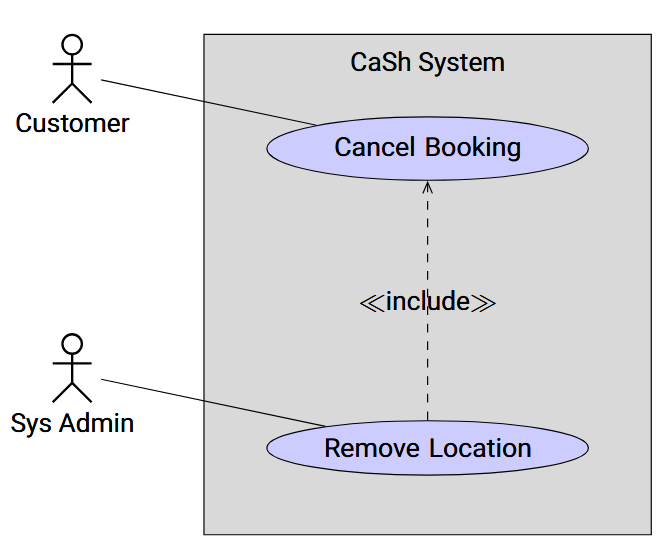
\includegraphics[scale=0.5]{Pics/03/UML_Include.png}
        \caption{UML Include}
    \end{minipage}
    \hfill
    \begin{minipage}
        [htp]{0.5\textwidth}
        \centering
        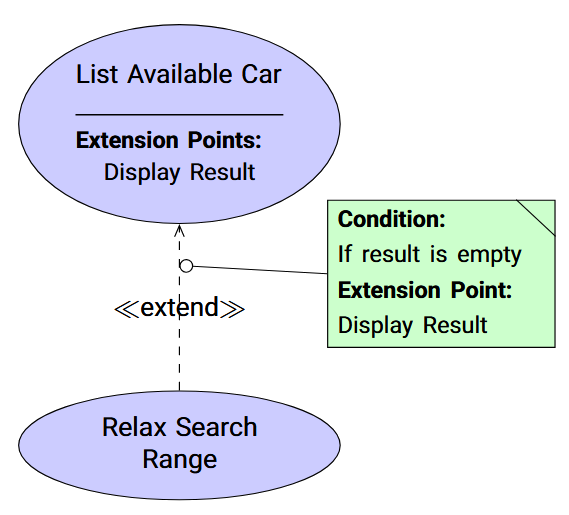
\includegraphics[scale=0.5]{Pics/03/UML_Extends.png}
        \caption{UML Extend}
    \end{minipage}
\end{figure}
\end{document}